\documentclass[aspectratio=169,xcolor=dvipsnames]{beamer}
% https://github.com/PM25/SimplePlus-BeamerTheme
\usetheme{SimplePlus}

\usepackage{hyperref}
\usepackage{graphicx} 
\usepackage{booktabs}
\usepackage{courier}

\usepackage[spanish]{babel}

% Portada

\title{\large Aplicación de técnicas de virtualización ligera para la evaluación de redes de comunicaciones}

\author{\small \textit{Autor}: Enrique Fernández Sánchez \\
\textit{Tutor}: José María Malgosa Sanahuja}

\institute[UPCT]{\\ Universidad Politécnica de Cartagena (UPCT) \\ \vspace{5px}
	
\includegraphics[scale=0.2]{img/escudo_upct.png}
}

\date{4 de abril de 2022}

\usepackage{tikz}
\logo{ 
	\begin{tikzpicture}[overlay,remember picture, inner sep=0pt,outer sep=0pt]
		\node[yshift=-20px,left=0.2cm] at (current page.31){
			
\includegraphics[width=3cm]{img/etsit.png}
		};
	\end{tikzpicture}
}

\begin{document}
	% 1
	\begin{frame}
		\titlepage
	\end{frame}

	% 2
	\begin{frame}{Índice}
		\tableofcontents
	\end{frame}
	
%	\begin{frame}{Índice de la memoria}
%	    \begin{enumerate}
%	        \item Introducción
%	        \item Virtualización de funciones de red
%	        \item Interfaces de red virtuales en Linux
%	        \item Espacio de nombres en Linux
%	        \item Virtualización ligera y contenedores
%	        \item Caso práctico: Virtualización para la simulación de redes
%	        \item Conclusiones
%	    \end{enumerate}
%	\end{frame}

    % --------------------
    \section{Introducción}
    
    \begin{frame}{Introducción}
    
        \begin{itemize}
            \item \textit{Abstract}: Guía ejemplificada para comprender los conceptos de virtualización ligera, contenedores y namespaces. 
        \end{itemize}
    
        \begin{block}{Objetivos del proyecto}
            \begin{itemize}
                \item Aprender \textbf{conceptos básicos de NFV}.
                \item \textbf{Diferenciar entre virtualización} ``dura'' y ``ligera''.
                \item Estudiar soluciones, dentro del sistema operativo Linux, que permitan realizar soluciones NFV.
                \item \textbf{Definir \textit{namespaces}}.
                \item Desgranar el \textbf{concepto de contenedor}.
                \item \textbf{Ejemplos de uso} de la virtualización ``ligera'' para la simulación de redes de telecomunicaciones.
            \end{itemize}
        \end{block}
    \end{frame}

	% ---------------------

	\section{Virtualización de funciones de red}
	
	\begin{frame}{Virtualización de funciones de red}
		\begin{itemize}
		    %\item Contextualización sobre la importancia de la virtualización en las redes.
		    \item \textit{Nacimiento de NFV}: \textit{white paper} en octubre de 2012 (WG de la ITU, 13 operadoras)
		    \item NFV como \textbf{solución para los problemas de las operadoras de red}
		\end{itemize}
		
		\begin{alertblock}{Problemas actuales de las operadoras de red}
		    \begin{itemize}
		        \item Saturación general en la red.
		        \item Dispositivos de red que requieren una instalación o intervención manual.
		        \item Problemas de gestión de las operadoras de red (ej: reducción de costes).
		    \end{itemize}
		\end{alertblock}
	\end{frame}
	
	\begin{frame}{Virtualización de funciones de red}
	    \begin{itemize}
	        \item Comparación entre redes clásicas y redes virtualizadas: 
	    \end{itemize}
	
	    \begin{columns}
	        % Columna 1
	        \begin{column}{0.5\textwidth}
	        \begin{exampleblock}{\textit{Classic networks}}
	            \begin{itemize}
	                \item Hardware embebido.
	                \item Cada \textbf{dispositivo} de red asociado a una \textbf{única función} de red (firewall, balanceador de carga, router...)
	                \item Software dependiente del ``vendor'' (cisco, jupyter...)
	                \item Gestión de recursos software/hardware limitada.
	            \end{itemize}
	        \end{exampleblock}
	        \end{column}
	        
	        % Columna 2
	        \begin{column}{0.5\textwidth}
	        \begin{exampleblock}{\textit{Network Functions Virtualization} (\texttt{NFV})}
	            \begin{itemize}
	                \item Hardware de carácter general.
	                \item Un \textbf{mismo hardware} puede tener asociadas \textbf{más de una función} de red.
	                \item Independencia del ``vendor''.
	                \item Gestión de recursos software/hardware total.
	            \end{itemize}
	        \end{exampleblock}
	        \end{column}
	    \end{columns}
	\end{frame}
	
	\begin{frame}{Virtualización de funciones de red}
	
	\begin{columns}
	% Columna 1
	\begin{column}{0.6\textwidth}
	    \begin{figure}[h]
            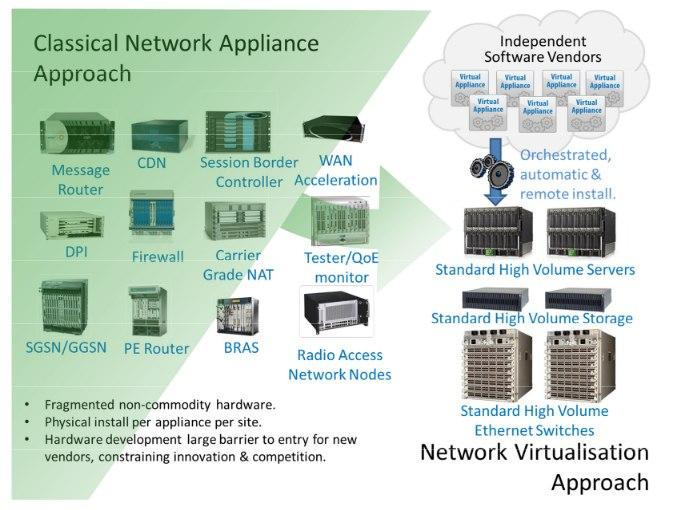
\includegraphics[width=0.95\textwidth]{img/classic_network_vs_nfv.jpg}
            \caption{Comparativa enfoque clásico contra enfoque virtualizado}
       \end{figure}
	\end{column}
	
	% Columna 2
	\begin{column}{0.4\textwidth}
	\begin{alertblock}{Ventajas de NFV}
	    \begin{itemize}
	        \item \textbf{Desacoplar funciones de red} de hardware específico.
	        \item Acelerar desarrollo de servicios para los operadores de red.
	        \item Reducción de costes.
	    \end{itemize}
	\end{alertblock}
	\end{column}
	\end{columns}
	
	\end{frame}
	
	\begin{frame}{SDN \& NFV}
        \begin{columns}
            \begin{column}{0.6\textwidth}
            \begin{alertblock}{\textit{Software Defined Networks} (\texttt{SDN})}
            \begin{itemize}
                \item NFV depende de SDN, y viceversa.
                \item SDN desacopla el plano de control y el plano de datos de hardware de red. 
                \item El \textbf{controlador SDN} es el encargado de gestionar el plano de control de los dispositivos.
                \item Un router solo sabe encaminar paquetes de la forma que el controlador SDN le ha programado.
            \end{itemize}
            \end{alertblock}
            
            \begin{block}{APIs implicadas en SDN}
                    Para programar bajo el paradigma SDN utilizamos:
                    \begin{itemize}
                        \item \texttt{Southbound}
                        \item \texttt{Northbound} 
                    \end{itemize}
            \end{block}
            \end{column}
            
            \begin{column}{0.4\textwidth}
                \begin{figure}[h]
                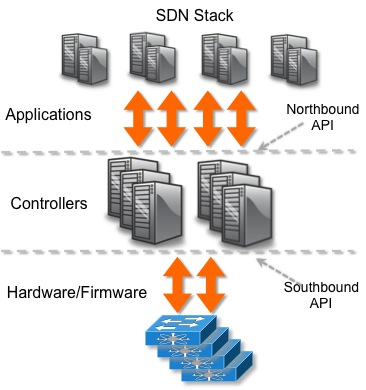
\includegraphics[width=0.95\textwidth]{img/south_north.jpg}
                \caption{Esquema y ámbito de aplicacion de las APIs}
                \end{figure}
            \end{column}
        \end{columns}
	\end{frame}
	
	\begin{frame}{Virtualización ``ligera''}
	\begin{columns}
	\begin{column}{0.4\textwidth}
	    \begin{block}{\textit{Lightweight virtualization}}
	        \begin{itemize}
	            \item El propio \texttt{kernel} del SO realiza la virtualización.
	            \item \textbf{Espacios} de usuarios \textbf{aislados} entre sí.
	            \item Conocida como \texttt{containers}.
	        \end{itemize}
	    \end{block}
	    
	    \begin{exampleblock}{Comparativa virt. ``dura''}
	        \begin{itemize}
	            \item Eliminamos el \textit{overhead}, al tener un único kernel.
	            \item Menor consumo de recursos.
	            \item Facilidad a la hora de manipular las instancias.
	        \end{itemize}
	    \end{exampleblock}
	\end{column}
	
	\begin{column}{0.6\textwidth}
	    \begin{figure}
            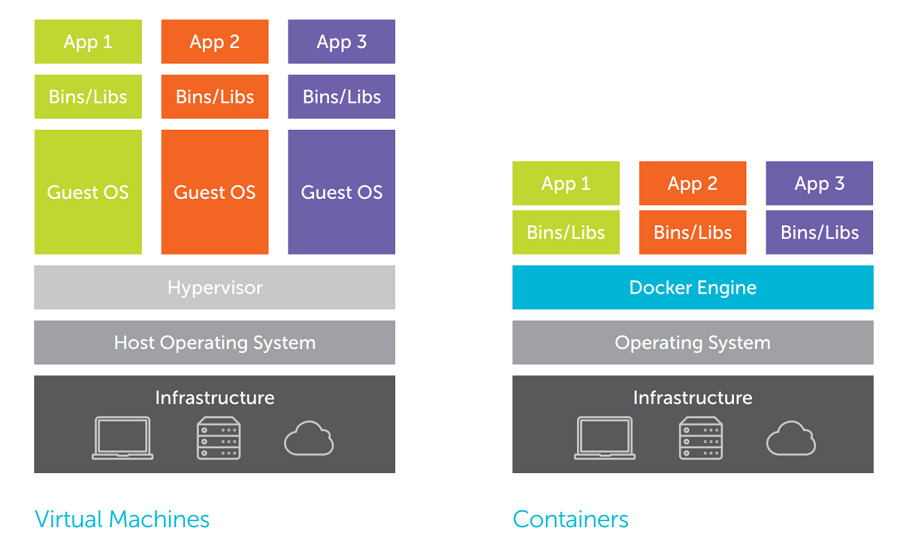
\includegraphics[width=1\textwidth]{img/virtualization_comparative_2.png}
            \caption{Comparativa entre virt. dura (izq.) y virt. ligera (der.)}
       \end{figure}
	\end{column}
	
	\end{columns}
	\end{frame}
	
	% ---------------------
	
	\section{Interfaces de red virtuales en Linux}
	
	\begin{frame}{Interfaces de red virtuales en Linux}
		\begin{itemize}
		    \item Linux permite una amplia \textbf{selección de interfaces virtuales de red}. Algunas de ellas son realmente interesantes \textbf{para la implementación de virtualización ligera}, ya que permiten comunicar las instancias aisladas.
		\end{itemize}
		
		\begin{alertblock}{Selección de interfaces de red virtuales en Linux}
		    \begin{itemize}
		        \item Bridge
		        \item MAC compartida
		        \item VLAN 802.1q
		        \item VLAN 802.1ad
		        \item \textbf{Pares ethernet virtuales}
		        \item \textbf{TUN/TAP}
		    \end{itemize}
		\end{alertblock}
	\end{frame}
	
	\begin{frame}{Pares ethernet virtuales}
	    \begin{columns}
	        \begin{column}{0.5\textwidth}
	                \begin{figure}[h]
                        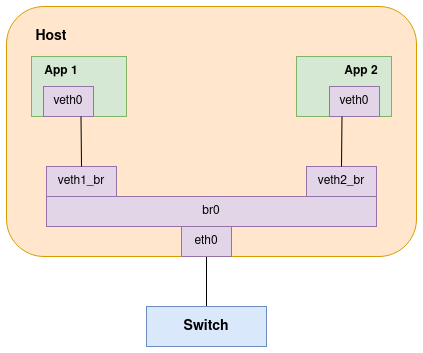
\includegraphics[width=0.95\textwidth]{img/veth_ej2.png}
                        \caption{Diagrama de ejemplo de uso de pares ethernet virtuales}
                    \end{figure}
	        \end{column}
	        
	        \begin{column}{0.5\textwidth}
	            \begin{block}{Ejemplo: topología usando veth}
	                \begin{itemize}
	                    \item \textbf{Dispositivos} virtuales \textbf{creados a pares}.
	                    \item Los paquetes transmitidos en un extremos se reciben automáticamente en el otro extremo.
	                    \item Útiles para asignar un extremo de la pareja a un \textbf{namespace}.
	                    \item \texttt{ip link add ... type veth peer ...}
	                \end{itemize}
	            \end{block}
	        \end{column}
	    \end{columns}
	\end{frame}
	
	\begin{frame}{TUN/TAP}
	    \begin{columns}
	        \begin{column}{0.5\textwidth}
	            Permiten conectar aplicaciones a través de un socket de red.
	            \begin{itemize}
	                \item TUN. Transporta paquetes IP
	                \item TAP. Transporta \textit{frames} Ethernet.
	            \end{itemize}
	            
	            \begin{exampleblock}{Crear interfaz TUN/TAP}
	                \begin{itemize}
	                    \item \texttt{tunctl}
	                    \item \texttt{ip tuntap}
	                \end{itemize}
	            \end{exampleblock}
	        \end{column}
	        
	        \begin{column}{0.5\textwidth}
	                \begin{figure}[h]
                        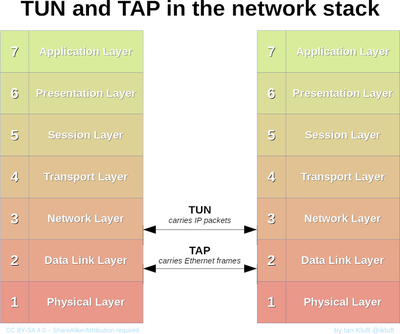
\includegraphics[width=1\textwidth]{img/tun_vs_tap.png}
                        \caption{Comparativa en capa OSI de TUN/TAP}
                    \end{figure}
	        \end{column}
	    \end{columns}
	\end{frame}
	
	\begin{frame}{Ejemplos interfaces de red virtuales}
	    \begin{alertblock}{Ejemplos realizados en esta sección de la memoria}
	        \begin{itemize}
	            \item Creación de cada una de las interfaces de red virtuales.
	            \item Aplicación que crea una interfaz TUN/TAP.
	            \item Aislamiento entre puertos usando interfaz TUN/TAP.
	        \end{itemize}
	    \end{alertblock}
	\end{frame}
	
	% ---------------------
	
	\section{Namespaces}
	
	\begin{frame}{Namespaces}
	
	    \begin{columns}
	    \begin{column}{0.6\textwidth}
	        \begin{block}{Definición namespace}
	           \textbf{Característica del kernel} de Linux que permite \textbf{gestionar} los recursos, \textbf{pudiendo limitarlos} a uno (o varios) \textbf{procesos}.
	           
	           \begin{itemize}
	               \item \textit{Objetivo}: adquirir una característica del sistema como una abstracción. Dentro del namespace tienen su propia \textbf{instancia aislada} del recurso global.
	           \end{itemize}
	        \end{block}
	        
	        \begin{alertblock}{Crear/acceder namespace}
	            \begin{itemize}
	                \item \texttt{unshare}
	                \item \texttt{nsenter}
	            \end{itemize}
	        \end{alertblock}
	    \end{column}
	    
	    \begin{column}{0.4\textwidth}
	        \begin{exampleblock}{¿Cuantos namespaces hay?}
		    \begin{enumerate}
		        \item UTS (\texttt{hostname})
		        \item \textbf{Mount}
		        \item Process ID
		        \item \textbf{Network}
		        \item User ID
		        \item Interprocess Communication
		        \item \textbf{Control groups}
		        \item \textbf{Time}
		    \end{enumerate}
		\end{exampleblock}
	    \end{column}
	    \end{columns}
	\end{frame}

% Eliminar transparencia
%    \begin{frame}{UTS - Process ID - User ID - IPC}
%        \begin{columns}
%        \begin{column}{0.5\textwidth}
%            \begin{block}{\centering Unix Time Sharing (UTS)}
%                    \begin{itemize}
%                        \item Controla el hostname asociado al proceso.
%                        %\item Uso: \\ \texttt{unshare -u /bin/sh \\ hostname <hst>}
%                    \end{itemize}
%            \end{block}
%            
%            \begin{block}{\centering Interprocess Communication (IPC)}
%                    \begin{itemize}
%                        \item Controla la comunicación entre procesos.
%                        \item Aplicación más compleja de los namespaces.
%                        \item Uso común en bases de datos.
%                    \end{itemize}
%            \end{block}
%        \end{column}
%        
%        \begin{column}{0.5\textwidth}
%            \begin{block}{\centering Process ID}
%                    \begin{itemize}
%                        \item Aísla el namespace de la ID del proceso asignado
%                        \item Dentro del namespace, el proceso piensa que tiene el ID ``1''
%                    \end{itemize}
%            \end{block}
%            
%            \begin{block}{\centering User ID}
%                    \begin{itemize}
%                        \item Permite ``mappear'' un UID/GID dentro del namespace, diferente al del host.
%                        \item Aunque dentro del namespace tengamos UID 0 (root), no tenemos acceso a los archivos root del host.
%                    \end{itemize}
%            \end{block}
%        \end{column}
%        \end{columns}
%    \end{frame}
    
    \begin{frame}{Mount namespace}
        \begin{itemize}
            \item Primer namespace en aparecer en el kernel.
            \item \textit{Objetivo}: \textbf{restringir la visualización} de la jerarquía \textbf{global} de archivos. Cada namespace tiene su \textbf{propio ``set''} de puntos de montaje.
        \end{itemize}
        
        \begin{alertblock}{\textit{Shared subtrees}}
        Por defecto, los mount namespaces tienen activada la opción de \texttt{shared subtree}. Esta opción determina \textbf{cómo se van a propagar los montajes} a otros puntos de montaje.
        \begin{itemize}
            \item \texttt{shared mount}. Replicado, todas las copias iguales.
            \item \texttt{slave mount}. Montaje tipo esclavo, solo se propagan hacia él.
            \item \texttt{private mount}. No permite propagación.
            \item \texttt{unbindeable mount}. No permite ser asociado.
        \end{itemize}
        \end{alertblock}
    \end{frame}
    
    \begin{frame}{Mount namespace}
        \begin{columns}
            \begin{column}{0.5\textwidth}
                \begin{itemize}
                    \item Un mount namespace nos \textbf{permite modificar un sistema de archivos} en concreto, \textbf{sin que otros procesos puedan ver y/o acceder} a dicho sistema de archivo.
                    \item Permite tener \textbf{diferentes vistas para cada namespace}.
                \end{itemize}
            \end{column}
        
            \begin{column}{0.5\textwidth}
                \begin{alertblock}{Montaje tipo bind}
                    Opción de \texttt{mount} (\texttt{--bind}) que nos permite realizar un \textbf{montaje} de un dispositivo \textbf{sobre un directorio} de nuestro sistema de archivos.
                \end{alertblock}
                
                \begin{alertblock}{Sistema de archivos temporal (\texttt{tmpfs})}
                    Funcionalidad que permite crear un \textbf{sistema de archivos temporal} dentro de nuestro sistema. El sistema creado se aloja en memoria.
                \end{alertblock}
            \end{column}
        \end{columns}
    \end{frame}
    
    \begin{frame}{Network namespace}
        \begin{itemize}
            \item Permite \textbf{aislar la red de un proceso}.
            \item El namespace crea una interfaz virtual, con un \textbf{stack de red completo}.
        \end{itemize}
        
        \begin{exampleblock}{Creación de network namespace}
            \begin{itemize}
                \item Para que el network namespace sea persistente, lo tenemos que crear con: \texttt{ip netns add <nombre>} o \texttt{unshare --net=<file>}
                \item Si quisiéramos comprobar los network namespaces existentes, ejecutamos: \texttt{ip netns} o \texttt{lsns}
                \item Para tener conectividad con el exterior, tenemos que añadirle una interfaz virtual: \texttt{veth}, \texttt{ip link set <veth link> netns <nombre>}
            \end{itemize}
        \end{exampleblock}
    \end{frame}
    
    \begin{frame}{Control groups \& time}
        \begin{columns}
            \begin{column}{0.5\textwidth}
                \begin{block}{Control groups (\texttt{cgroups})}
                    \begin{itemize}
                        \item \textbf{Mecanismos de control} para los recursos del sistema.
                        \item Funcionalidades que puede realizar:
                        \begin{itemize}
                            \item Limitar recursos
                            \item Priorizar tareas
                            \item Monitorización
                            \item Control
                        \end{itemize}
                        \item \textbf{Configurado utilizando sistema de archivos virtual}: \texttt{/sys/fs/cgroup}
                        \item Disponibles dos versiones: cada vez más aceptada la \texttt{v2}
                    \end{itemize}
                \end{block}
            \end{column}
        
            \begin{column}{0.5\textwidth}
                \begin{block}{Time}
                    \begin{itemize}
                        \item Último namespace añadido al kernel
                        \item Permite \textbf{crear desfases entre los relojes del sistema}.
                        \item Cambiar la fecha y hora dentro del namespace sin modificar la del host.
                    \end{itemize}
                \end{block}
            \end{column}
        \end{columns}
    \end{frame}
	
	\begin{frame}{Ejemplos namespaces}
	    \begin{alertblock}{Ejemplos realizados en esta sección de la memoria}
	        \begin{columns}
	        \begin{column}{0.5\textwidth}
	            \begin{itemize}
	                \item Uso de UTS namespace
	                \item \textbf{Persistencia de un namespace}
	                \item Mount namespace con dispositivo físico
	                \item \textbf{Casos de uso de montaje tipo bind}
	                \item \textbf{Casos de uso de shared subtree}
	                \item \textbf{Topología de red usando network namespaces y NAT}
	            \end{itemize}
	        \end{column}
	        
	        \begin{column}{0.5\textwidth}
	            \begin{itemize}
	                \item Uso de process ID namespace
	                \item Uso de UID namespace
	                \item \textbf{Limitar memoria RAM con cgroups}
	                \item \textbf{Limitar uso de CPU con cgroups}
	                \item Topología de red usando comando \texttt{ip}
	                \item Topología de red usando comando \texttt{unshare}
	            \end{itemize}
	        \end{column}
	    \end{columns}
	    \end{alertblock}
	\end{frame}
	
	% ---------------------
	
	\section{Virtualización ligera y contenedores}
	
	\begin{frame}{Virtualización ligera y contenedores}
		\begin{block}{Definición virt. ligera}
		    Tipo de virtualización que se realiza a \textbf{nivel de sistema operativo}, permitiendo la \textbf{coexistencia de diferentes espacios aislados} entre sí. Todas las instancias aisladas \textbf{utilizan el mismo kernel}. 
		\end{block}
		
		\begin{block}{Definición contenedor}
		    \textbf{Abstracción alto nivel de un sistema aislado} creado utilizando \texttt{namespaces} y \texttt{cgroups}. Además, proporcionan unas \textbf{APIs de alto nivel} para interactuar con el contenedor. Algunos ejemplos de sistemas de contenedores son:
		    
		    \begin{itemize}
		        \item \texttt{LXC}, LinuX Containers.
		        \item \texttt{Docker}
		        \item \texttt{Podman}
		    \end{itemize}
		\end{block}
	\end{frame}
	
	\begin{frame}{Contenedor DIY}
	    \begin{itemize}
	        \item Fundación \textit{Linux Foundation's Container Initiative} (\texttt{OCI}) recoge las directivas para crear \texttt{images} y \texttt{runtimes}.
	        \item Diferentes \texttt{runtimes} en función de la solución de contenedores a utilizar.
	        
	        \begin{columns}
	                \begin{column}{0.5\textwidth}
	                \begin{exampleblock}{\texttt{Images}}
	                    \begin{itemize}
	                        \item Contiene un \textbf{sistema de archivos root} con las dependencias de la aplicación.
	                        \item Imágenes diferenciadas en capas, que serán montadas por el \texttt{runtime} usando \textit{montajes de unión}. (\texttt{overlayfs})
	                        \item Capa inferior inmutable y capa superior con todo lo referido a la aplicación.
	                    \end{itemize}
	                \end{exampleblock}
	                \end{column}
	                
	                \begin{column}{0.5\textwidth}
	                \begin{exampleblock}{\texttt{Runtimes}}
	                    \begin{itemize}
	                        \item Dada una imagen, \textbf{\texttt{runtime} la ejecutará}.
	                        \item Creación y configuración de los namespaces (netns, pid, ipc, uts, etc).
	                        \item Configuración de cgroups para monitorización y limites de recursos.
	                        \item Montaje de las ``capas'' del sistema de archivos.
	                    \end{itemize}
	                \end{exampleblock}    
	                \end{column}
	        \end{columns}
	    \end{itemize}
	\end{frame}
	
	\begin{frame}{LXC}
	    \begin{columns}
	        \begin{column}{0.6\textwidth}
	            \begin{itemize}
	                \item Contenedores de \textbf{bajo nivel}. Uso de \texttt{mount namespaces} para conseguir una \textbf{estructura de directorios} propia de una \textbf{distribución de Linux}.
	                \item Virtualización de una \textbf{distribución completa}.
	                \item Permite crear contenedores sin privilegios, es decir, no pueden realizar acciones sobre el host.
	                \item Apto para la ejecución de entornos gráficos.
	                \item Galería de imágenes: \url{https://uk.lxd.images.canonical.com/}
	            \end{itemize}
	        \end{column}
	        
	        \begin{column}{0.4\textwidth}
	            \begin{figure}[h]
                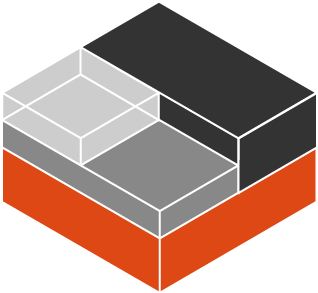
\includegraphics[width=0.8\textwidth]{img/lxc_logo.png}
                \caption{Logotipo \texttt{LXC}}
                \end{figure}
	        \end{column}
	    \end{columns}
	\end{frame}
	
	\begin{frame}{Docker}
	    \begin{figure}[h]
        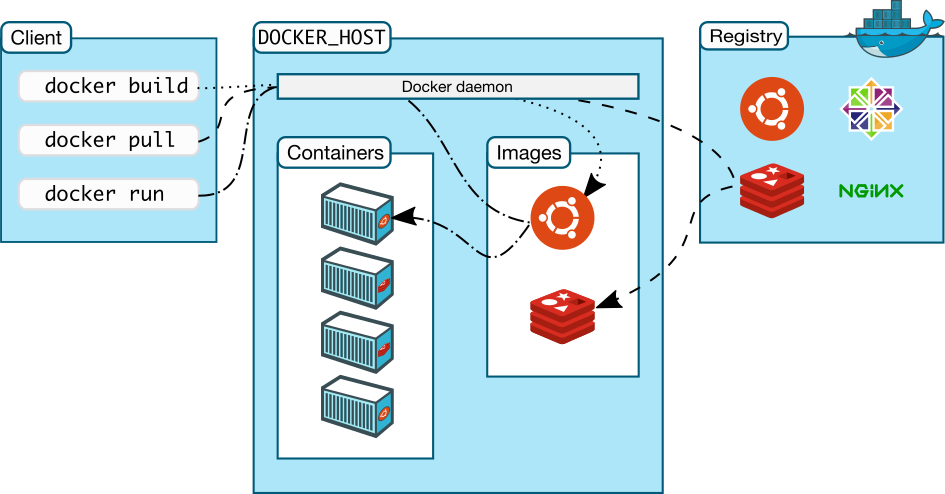
\includegraphics[width=0.6\textwidth]{img/architecture-docker.png}
        \caption{Arquitectura Docker}
        \end{figure}
	    
	    \begin{itemize}
	        \item Solución muy famosa de contenedores. Escrita en \texttt{Go}. Uso de \texttt{namespaces}.
	        \item \textbf{Arquitectura cliente-servidor}. Cliente se comunica con ``servicio'' para crear, ejecutar y distribuir los contenedores. 
	    \end{itemize}
	\end{frame}

    \begin{frame}{Ejemplos virtualización ligera}
        \begin{alertblock}{Ejemplos realizados sobre contenedores DIY}
            \begin{itemize}
                \item Análisis de imagen basada en \texttt{alpine}.
                \item Análisis del \texttt{runtime} para ejecutar aplicación usando imagen basada en \texttt{alpine}.
            \end{itemize}
        \end{alertblock}
        
        \begin{alertblock}{Ejemplos realizados sobre LXC}
	        \begin{itemize}
	            \item \textbf{Comprobar los namespaces de un contendor LXC en Ubuntu}
	        \end{itemize}
	    \end{alertblock}
    
         \begin{alertblock}{Ejemplos realizados sobre Docker}
	        \begin{itemize}
	            \item Primeros pasos
	            \item Crear un Dockerfile
	            \item \textbf{Comprobar los namespaces asociados a un contenedor Docker}
	        \end{itemize}
	    \end{alertblock}
    \end{frame}
    
	% ---------------------
	
	\section{Caso práctico: Virtualización para la simulación de redes}
	
	\begin{frame}{Virtualización para simulación de redes}
		\begin{itemize}
		    \item \textit{Objetivo}: evaluar y/o \textbf{simular situaciones} concretas de nuestras \textbf{redes}. Modelamos los nodos utilizando contenedores.
		\end{itemize}
		
		\begin{block}{Opciones para la evaluación y/o simulación de redes}
		    \begin{itemize}
		        \item \texttt{Shell script} para desplegar los namespaces necesarios para la topología. Uso de comandos \texttt{nsenter} y \texttt{unshare}.
		        
		        \item Desplegar e interconectar contenedores LXC. Cada contenedor con una función de red asociada.
		        
		        \item Utilizar un \textbf{simulador de redes basado en namespaces}. \textbf{Mininet} es un simulador que permite crear una red virtual realista utilizando namespaces. Permite un \textbf{sencillo uso} y un \textbf{despliegue rápido}.
		    \end{itemize}
		\end{block}
	\end{frame}
	
	\begin{frame}{Mininet}
	    \begin{itemize}
	        \item Permite customizar y \textbf{desplegar topologías de red fácilmente}.
	        \item Python API muy bien documentada.
	        \item \textbf{Herramienta muy utilizada} en el campo de la investigación, sobre todo en el ámbito de \textbf{SDN}.
	        \item Permite la integración de controladores SDN externos.
	    \end{itemize}
	
	    \begin{alertblock}{Ejemplos realizados con mininet}
	        \begin{itemize}
	            \item Primeros pasos
	            \item Topología simple sin mininet
	            \item Topología simple con mininet
	            \item Limitación de recursos, tanto en nodos como en enlaces
	            \item Controlador SDN externo: \texttt{Ryu}
	        \end{itemize}
	    \end{alertblock}
	\end{frame}
	
	\begin{frame}{Containernet}
	
	    \begin{columns}
	        \begin{column}{0.6\textwidth}
	        \begin{itemize}
	            \item Fork de \texttt{mininet}.
	            \item Permite añadir a la topología \textbf{contenedores Docker como hosts}.
	            \item Cambios dinámicos a la topología (añadir, conectar y eliminar contenedores).
	            \item Ejecución de comandos dentro de los contenedores usando Python API.
	            \item Limitar uso de recursos de los contenedores.
	        \end{itemize}
	        
	        \begin{alertblock}{Ejemplos realizados con containernet}
	        \begin{itemize}
	            \item Instalación y primeros pasos
	            \item Ejecución topología simple (dos contenedores, dos switchs y un controlador)
	        \end{itemize}
	        \end{alertblock}
	        \end{column}
	        
	        \begin{column}{0.4\textwidth}
	        \begin{figure}[h]
            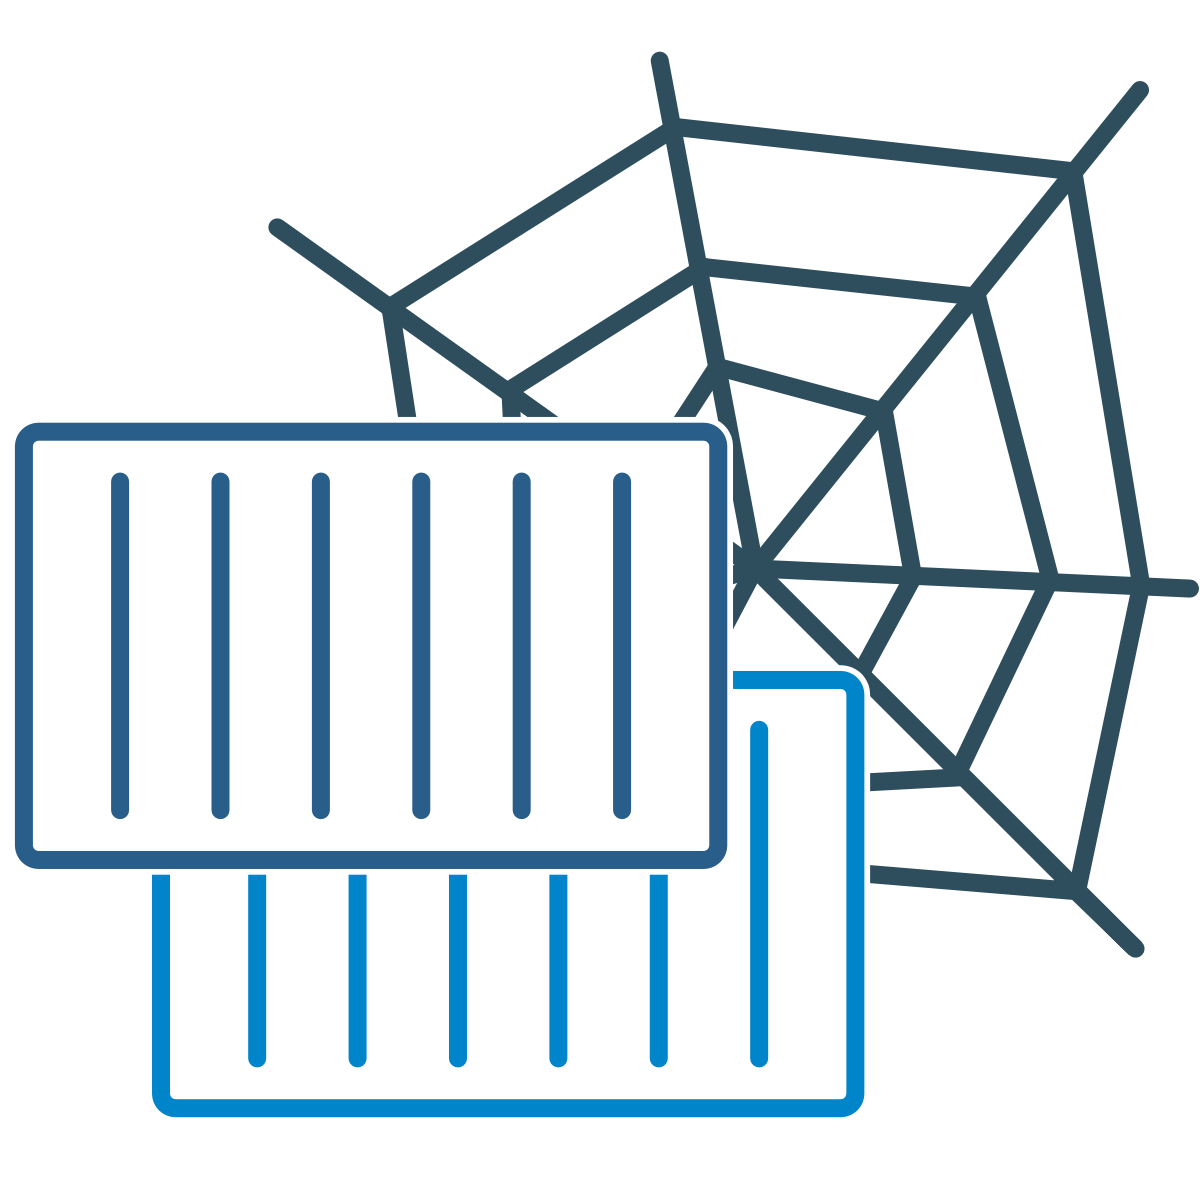
\includegraphics[width=0.7\textwidth]{img/containernet_logo.png}
            \caption{Logotipo \texttt{containernet}}
            \end{figure}
	        \end{column}
	    \end{columns}
	\end{frame}

	% ---------------------
	
	\section{Conclusiones}
	
	\begin{frame}{Conclusiones}
		\begin{itemize}
		    \item Alcanzados todos los objetivos propuestos
		    \item Se ha profundizado en el \textbf{concepto} de \textbf{contenedor} y \textbf{namespaces}
		    \item Se han realizado \textbf{28 ejemplos} sobre técnicas de \textbf{virt. ligera}
		    \item Se han aportado dos soluciones para la evaluación de redes de comunicaciones
		\end{itemize}
		
		\begin{exampleblock}{Propuestas futuras}
		    \begin{itemize}
		        \item Profundizar en las diferencias de rendimiento entre una virt. ``ligera'' y virt. ``dura''.
		        \item Investigar sobre modificaciones del protocolo OpenFlow. Además, indagar sobre \textbf{DPDK} y sus ventajas.
		        \item Pruebas de concepto del \textbf{lenguaje de programación P4}.
		    \end{itemize}
		\end{exampleblock}
	\end{frame}

	% ---------------------
	
	\section{Bibliografía}
	
	\begin{frame}{Bibliografía}
		\begin{itemize}
		    \item La contenida en la memoria del proyecto: páginas 100 - 102
		\end{itemize}
	\end{frame}
	
	\begin{frame}
	    \begin{center}
	        \vspace{30px}
	        \Large \textbf{Muchas gracias por su atención} \\
	        \vspace{30px}
	        \large ¿Preguntas? \\
	        \vspace{60px}
	        Enlace al proyecto: \small \url{https://github.com/Raniita/lightweight-virtualization-nfv}
	    \end{center}
	\end{frame}
	
\end{document}